\documentclass{article}
\usepackage[utf8]{inputenc}
\usepackage{amsfonts, amsmath, amssymb, dsfont, amssymb,mathtools, multirow, tikz}
% \usepackage{hyperref}



\title{Entropy}
\author{Sumit Singh}
\date{\today}

\begin{document}

\maketitle

\section{Equations}

\begin{align*}
  I(E) &= - \log[Pr(E)] = - \log(P)  \tag{Information}\\
  H(X) &= \mathbb{E}[I(X)] = \mathbb{E}[-log(P(X)] = - \sum_{i=1}^n P(x_i) \log P(x_i)  \tag{Entropy}\\
  D_{KL}(P||Q) &= \sum_{i=0}^n p(x_i) \log (p(x_i)) - \sum_{i=0}^n p(x_i) log(q(x_i)) \tag{KL Divergence}\\
  H(p,q) &= H(p) + D_{KL}(p||q) = -\sum_{i=0}^n p(x_i) log(q(x_i)) \tag{Cross Entropy}
\end{align*}

\section{Information}
\section{Gini}
\begin{equation*}
    Gini = 1 - \sum_{i=1}^n (p_i)^2
\end{equation*}
\section{Entropy}
Entropy ranges from 0 to 1, where 0 is a pure sub-tree and 1 is the most impure sub-tree. \\
Entropy for a fair sided die:\\
\begin{equation*}
    H = - \sum_{i=1}^6 \frac{1}{6} \log_2 (\frac{1}{6}) = \log_2(6) bits
\end{equation*}
\begin{tabular}{|c|c|c|}
  \hline
  \multicolumn{2}{|c|}{\textbf{Play Golf}}\\
  \hline
   $Yes$       & $No$       \\
  \hline
   $9$       & $5$       \\
  \hline 
\end{tabular}

\begin{align*}
    Entropy(Play Golf) &= Entropy(5,9) \\
    &= Entropy(0.36,0.64) \\
    &= -(0.36 \log_2 0.36) - (0.64 \log_2 0.64) \\
    &= 0.94
\end{align*}
\newpage  
\begin{figure}
  \centering
  \documentclass{standalone}
\usepackage{tikz}
\usetikzlibrary{positioning}
\newdimen\nodeDist
\nodeDist=35mm
\begin{document}

\begin{tikzpicture}[
    node/.style={%
      draw,
      rectangle,
    },
  ]

    \node [node] (A) {Root Node \{A\} 7 Yes, 5 No};
    \path (A) ++(-135:\nodeDist) node [node] (B) {\{B\} 2 Yes, 4 No};
    \path (A) ++(-45:\nodeDist) node [node] (C) {\{C\} 5 Yes, 1 No};

    \draw (A) -- (B) node [left,pos=0.25] {no}(A);
    \draw (A) -- (C) node [right,pos=0.25] {yes}(A);
\end{tikzpicture}

\end{document} 
  \caption{The enhanced diagram}
\end{figure}
\begin{align*}
    Entropy(B) &= - \frac{2}{2+4} \log_2 \frac{2}{2+4} - \frac{4}{4+2} \log_2 (\frac{4}{4+2})\\
               &= -\frac{1}{3} \log_2(\frac{1}{3}) - \frac{2}{3} \log_2(\frac{2}{3}) \\
               &= \frac{\log_2(3)}{3} + \frac{2 \log_2(1.5)}{3} \\
               &= 0.92 bits\\ 
    Entropy(C) &= - \frac{5}{6} \log_2(\frac{5}{6}) - \frac{1}{6} \log_2(\frac{1}{6}) \\
               &= \frac{5 \log_2(1.2)}{6} + \frac{\log_2(6)}{6}\\
               &= 0.65 bits
\end{align*}
    
%*********************************************************************************************   
\section{Kullback-Leibler (KL) Divergence}
%*********************************************************************************************   




%*********************************************************************************************   
\section{Cross Entropy}
%*********************************************************************************************   
The cross-entropy formula takes in two distributions, $p(x)$, the true distribution, and $q(x)$, the estimated distribution, defined over the discrete variable $s$ and is given by:
\begin{align*}
    H(p,q)  &= - \sum_{\forall x} p(x) log(q(x)) \\
            &= -p(x_1)log(q(x_1))-p(x_2)log(q(x_2))- \cdots -p(x_n)log(q(x_n))
\end{align*}
Taking the derivative with respect to some $x_i$:
\begin{align*}
    \frac{\partial}{\partial x_i} H(p,q) &= - \frac{\partial}{\partial x_i} p(x_i) log(q(x_i)) \\
    &= - \frac{p(x_i)}{q(x_i)} \frac{\partial q(x_i)}{\partial x_i}
\end{align*}





%*********************************************************************************************   
\subsubsection{Examples}
Example 1: \\
Actual Probabilities: [0 ,1, 0, 0] \\
Predicted Probabilities: [0.21, 0.68, 0.09, 0.10] \\
Cross Entropy  $ = -1 \times log(0.68) = 0.167 $ \\
Example 2: \\
Actual Probabilities: [0 ,1, 0, 0] \\
Predicted Probabilities: [0.21, 0.68, 0.09, 0.10] \\
Cross Entropy  $ = -1 \times log(0.68) = 0.167 $ \\
\begin{center}
    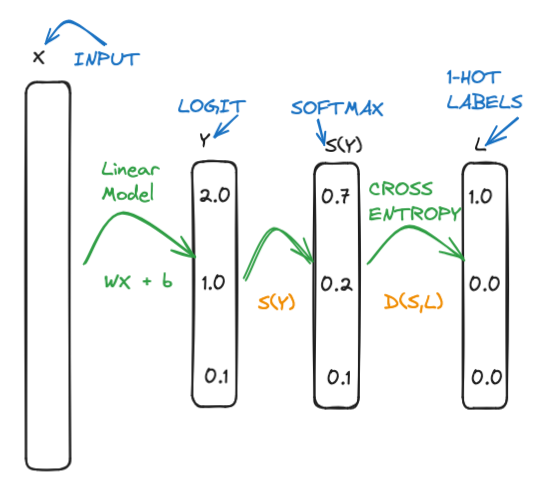
\includegraphics[width=9cm, height=6cm]{Topics/IMAGES/CrossEntropy1.png} 
\end{center}
\begin{align*}
    S(Y) &= f(s_i) &&= \frac{e^{s_i}}{\sum_j^C e^{s_j}} \\
    CE &= D(S,L) &&= - \sum_i L_i \log(S_i)
\end{align*}
\begin{itemize}
    \item \textbf{Entropy} calculates the degree of randomness or disorder within a system to measure the uncertainty of an event. If an outcome is certain, the measure of entropy will be low.
    \item \textbf{Cross-entropy} is used to measure the performance of a classification model.  It measures the difference between the discovered probability distribution of a classification model and predicted values. 
    \item \textbf{Binary cross-entropy} is used when performing binary classification, and \textbf{categorical cross-entropy} is used for multi-class classification.
    \item \textbf{Cross-entropy is similar to KL divergence}, but they serve different purpose: cross entropy is typically used in machine learning to evaluate the performance of a model when the objective is to minimize the error between the predicted probability distribution and true distribution, whereas KL is more useful in unsupervised learning tasks where the objective is to uncover structure in data by minimizing the divergence between the true and learned data distribution. 
    \item In both binary and multi-class classification, cross-entropy loss calculates how close the predicted probabilities are to the true label.
    \item Lower loss value indicates better performance
\end{itemize}
%*********************************************************************************************   
\section{Softmax}
%*********************************************************************************************   
\begin{equation*}
    S(y_i) = \frac{e^{y_i}}{\sum e^{y_i}}
\end{equation*}


\textbf{Softmax vs Sigmoid} \\
Softmax really wants to choose between one of the classes. It will always give max probability for one class. Sigmoid "neurons" may get activated for multiple claases. If the labels are mutually exclusive then softmax works better. Cross-entropy loss is softmax. Binary cross-entropy loss is sigmoid. 
%*********************************************************************************************   
\section{More Questions}
%********************************************************************************************* 
\textbf{Question}: Given the probability table below where $X$ represents the probability of you having a good or bad date and $Y$ represents the potential topics you could talk about during a date: \\ 
\begin{center}
\begin{tabular}{ c| c c }
       & x = good & x = bad \\ 
 \hline
 y = ex & 0.1 & 0.1 \\  
 y = food & 0.2 & 0.1 \\    
 y = travel & 0.4 & 0.1 \\
 \hline
\end{tabular}
\end{center}
\begin{itemize}
    \item Calculate the mutual information $I(X,Y)$
    \item Calculate the information (in base 2), given you had a bad date.
    \item Calculate the cross entropy between $p(x|y =  food)$ and $p(x|y = ex)$
    \item Calculate the KL divergence between $p(x|y = food)$ and $p(x|y = ex)$
    \item What is the information gain of $Y$ given $X$? 
\end{itemize}

%********************************************************************************************* 
\section{Neural network building blocks}
%********************************************************************************************* 

%********************************************************************************************* 
\subsection{The Machine Learning Method}
\begin{itemize}
    \item Define your model - which neural network, what does it output? ...
    \item Define your loss function - which parameters are good vs bad?
    \item Define your optimizer - how do we find good parameters?
\end{itemize}


%********************************************************************************************* 
\subsection{Negative log likelihood loss}
\begin{itemize}
    \item How is the negative log likelihood loss function motivated from maximum likelihood estimation?
    \item Why ius 
\end{itemize}

%********************************************************************************************* 
\subsection{Adam}
\begin{itemize}
    \item Basic idea: combine momentum with a second moment adjustment
\end{itemize}


%********************************************************************************************* 
\subsection{Input Standardization}


%********************************************************************************************* 
\subsection{Batch Normalization(BN)}
\begin{itemize}
    \item BN refers to normalizing $z^{(l)}$ or $a^{l}$ using statistics computed from the mini batch.
    \item We can think of this as putting a BN "layer" either before or after the nonlinearity.
    \item The BN layer also includes learnable scale and shift parameters.
    \item Model with BN layers operate in two different modes: "train" vs. "test" (or "eval")
    \begin{itemize}
        \item Train mode: compute statistics using the mini batch
        \item Eval mode: use an exponential moving average of the statistics computed during train time
    \end{itemize}
\end{itemize}
\begin{center}
    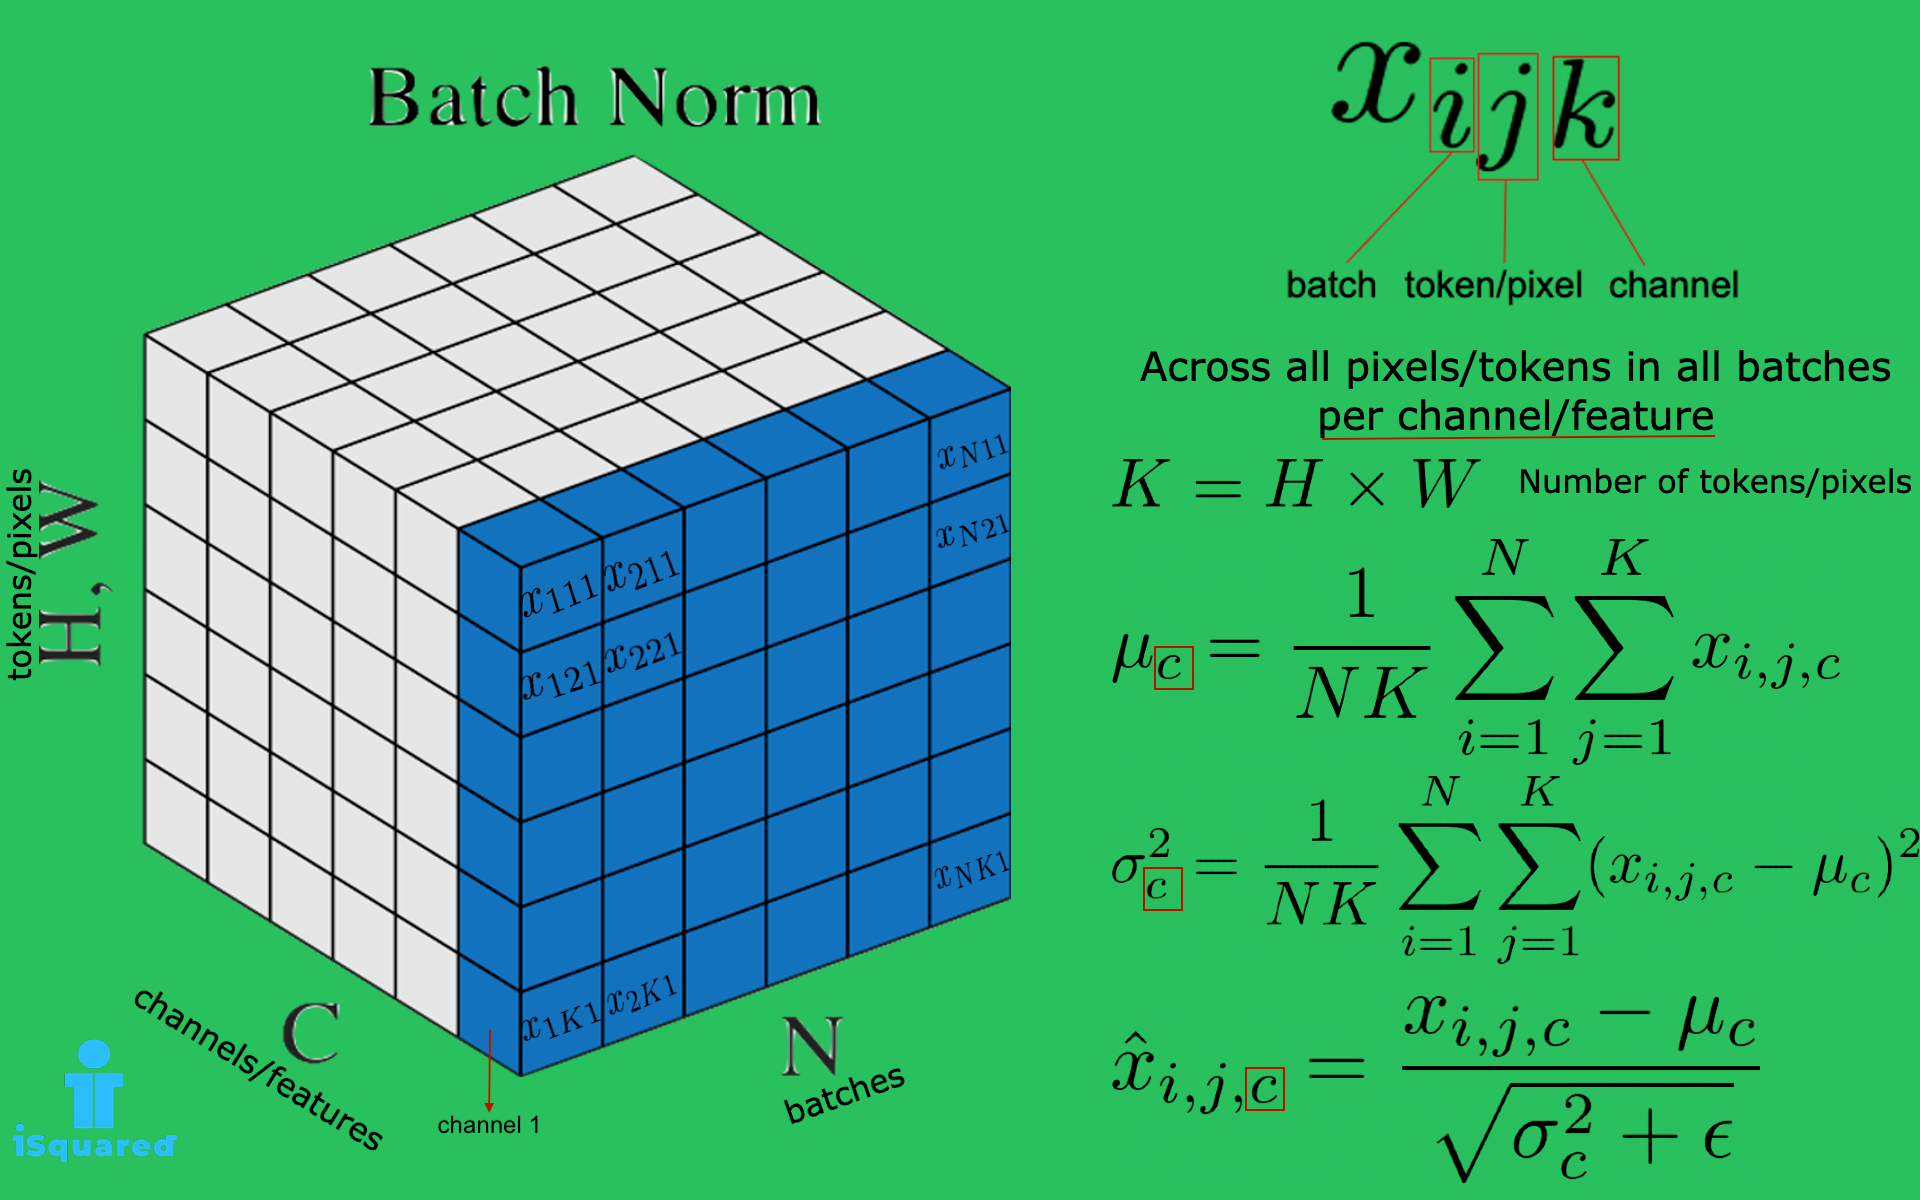
\includegraphics[width=9cm, height=6cm]{Topics/IMAGES/illustrated_batch_norm.png} 
\end{center}

%********************************************************************************************* 
\subsection{Layer Normalization (LN)}
\begin{center}
    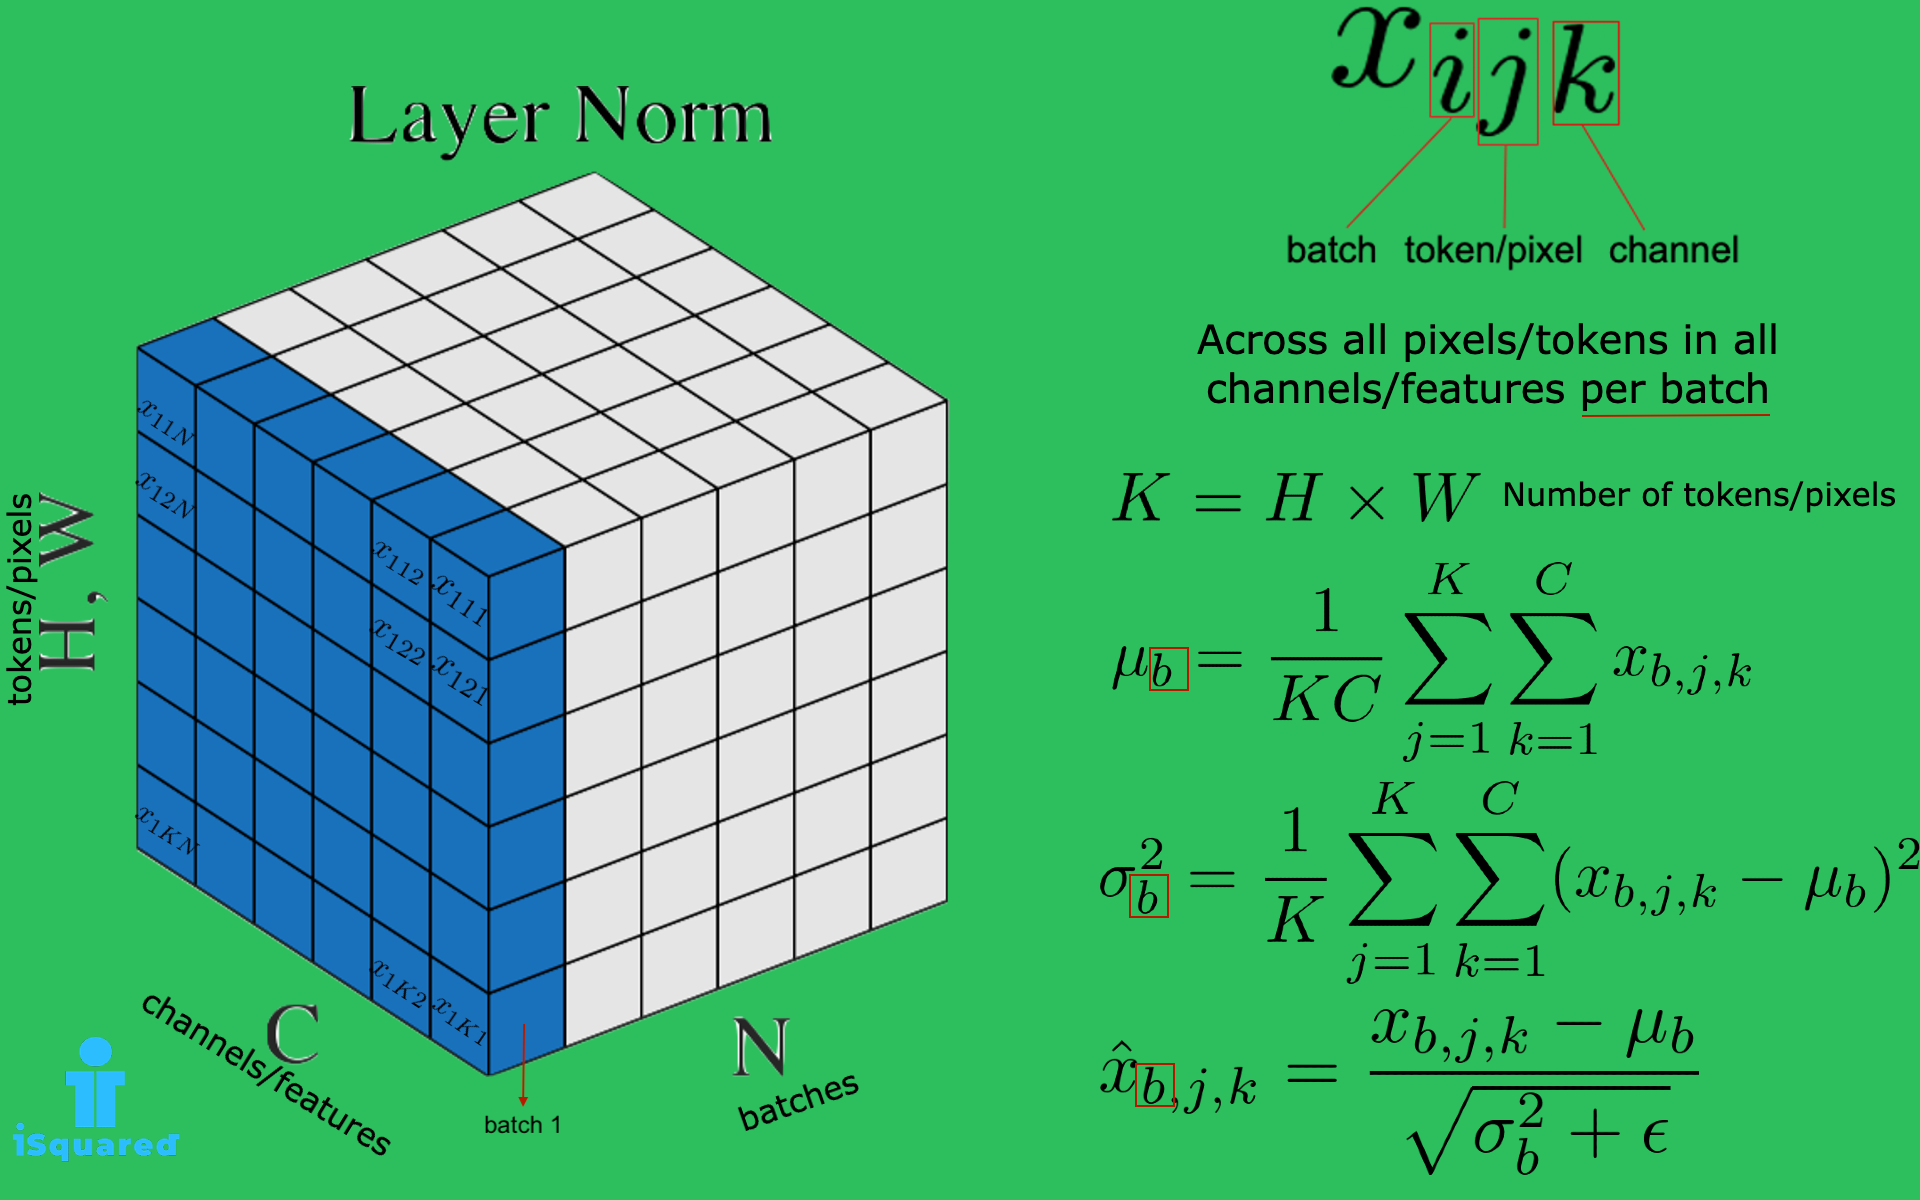
\includegraphics[width=9cm, height=6cm]{Topics/IMAGES/illustrated_layer_norm.png} 
\end{center}
\begin{itemize}
    \item LN is basically the "transpose" of BN: compute the mean and sd of $z^{(l)}$ across the feature dimensions, rather than per dimension.
    \begin{itemize}
        \item Now, each data point will have different normalization statistics, but these statistics are shared across dimensions
    \end{itemize}
    \item How is LN different from BN? How is it similar?
    \item What are the tradeoffs of BN vs LN?
    \item What are their shared benefits or downsides?
\end{itemize}


%********************************************************************************************* 
\subsection{Comparing different common nonlinearities}


%********************************************************************************************* 
\subsection{Skip Connections}


%********************************************************************************************* 
\subsection{Weight Initialization}


%********************************************************************************************* 
\subsection{Dropout}


%********************************************************************************************* 
\subsection{Data Augmentations}


%********************************************************************************************* 
\subsection{Neural network ensembles}

%********************************************************************************************* 
\section{Hyperparameter optimization}


\section{LLM}
\section{Developing an LLM - Build, Training, Fine-Tuning}
\subsection{RAG}
\subsection{Fine Tuning Embedding Models}
\subsection{Prompt Engineering vs RAG vs Fine-Tuning}

%********************************************************************************************* 
%********************************************************************************************* 
%********************************************************************************************* 
\section{References}
\begin{itemize}
    \item \href{https://www.datacamp.com/tutorial/the-cross-entropy-loss-function-in-machine-learning}{Kurtis Pykes}
    \item \href{https://www.geeksforgeeks.org/cross-entropy-cost-functions-used-in-classification/}{geeks for geeks}
    \item \href{https://isquared.digital/blog/2023-03-15-illustrated-batch-vs-layer-norm/}{Vladimir Ilievski}
    \item \href{https://www.youtube.com/watch?v=ALm-nzS0if4}{Chieh Wu}
    \item \href{https://cs182sp22.github.io/assets/lecture_slides/2022.02.28-mt1-review.pdf}{CS182 282A}
    
\end{itemize}
\end{document}